\documentclass{beamer}
\usetheme{Rochester}
\usecolortheme{beetle}
\usepackage{graphicx}
\usepackage{color}

%========aliases====================%
\newcommand{\bsym}{\boldsymbol}
\newcommand{\non}{\nonumber}

%========Title Page attributes====================%
\title[Torus]
{QHE in Torus Geometry}
\subtitle{Notes on symmetries}

\author[Abhishek]
{A.~Anand\inst{1}}

\institute[IISERP]
{
  \inst{1}%
  Indian Institute of Science Education and Research\newline
  Pune
}
\date{Jan 21, 2021}
\subject{Physics}

%========toc before each section====================%

\AtBeginSection[]
{
  \begin{frame}
    \frametitle{Table of Contents}
    \tableofcontents[currentsection]
  \end{frame}
}

%========Doc begin====================%

\begin{document}
	\begin{frame}[plain] \titlepage \end{frame} 
	\begin{frame}                                                                                                                                                        
    		\frametitle{Table of Contents}
    		\tableofcontents[currentsection]                                                                                                                                
	\end{frame} 
	
	\section{Introduction}

	%===============Intro>Intro====================%	
	
	\begin{frame}[noframenumbering,allowframebreaks]{Introduction}
  		Working in torus geometry is equivalent to imposing periodic boundary conditions on a parallelogram unit 				cell along both its lattice vectors. Say we have following parallelogram :

 		 \begin{figure}
    			\centering
    			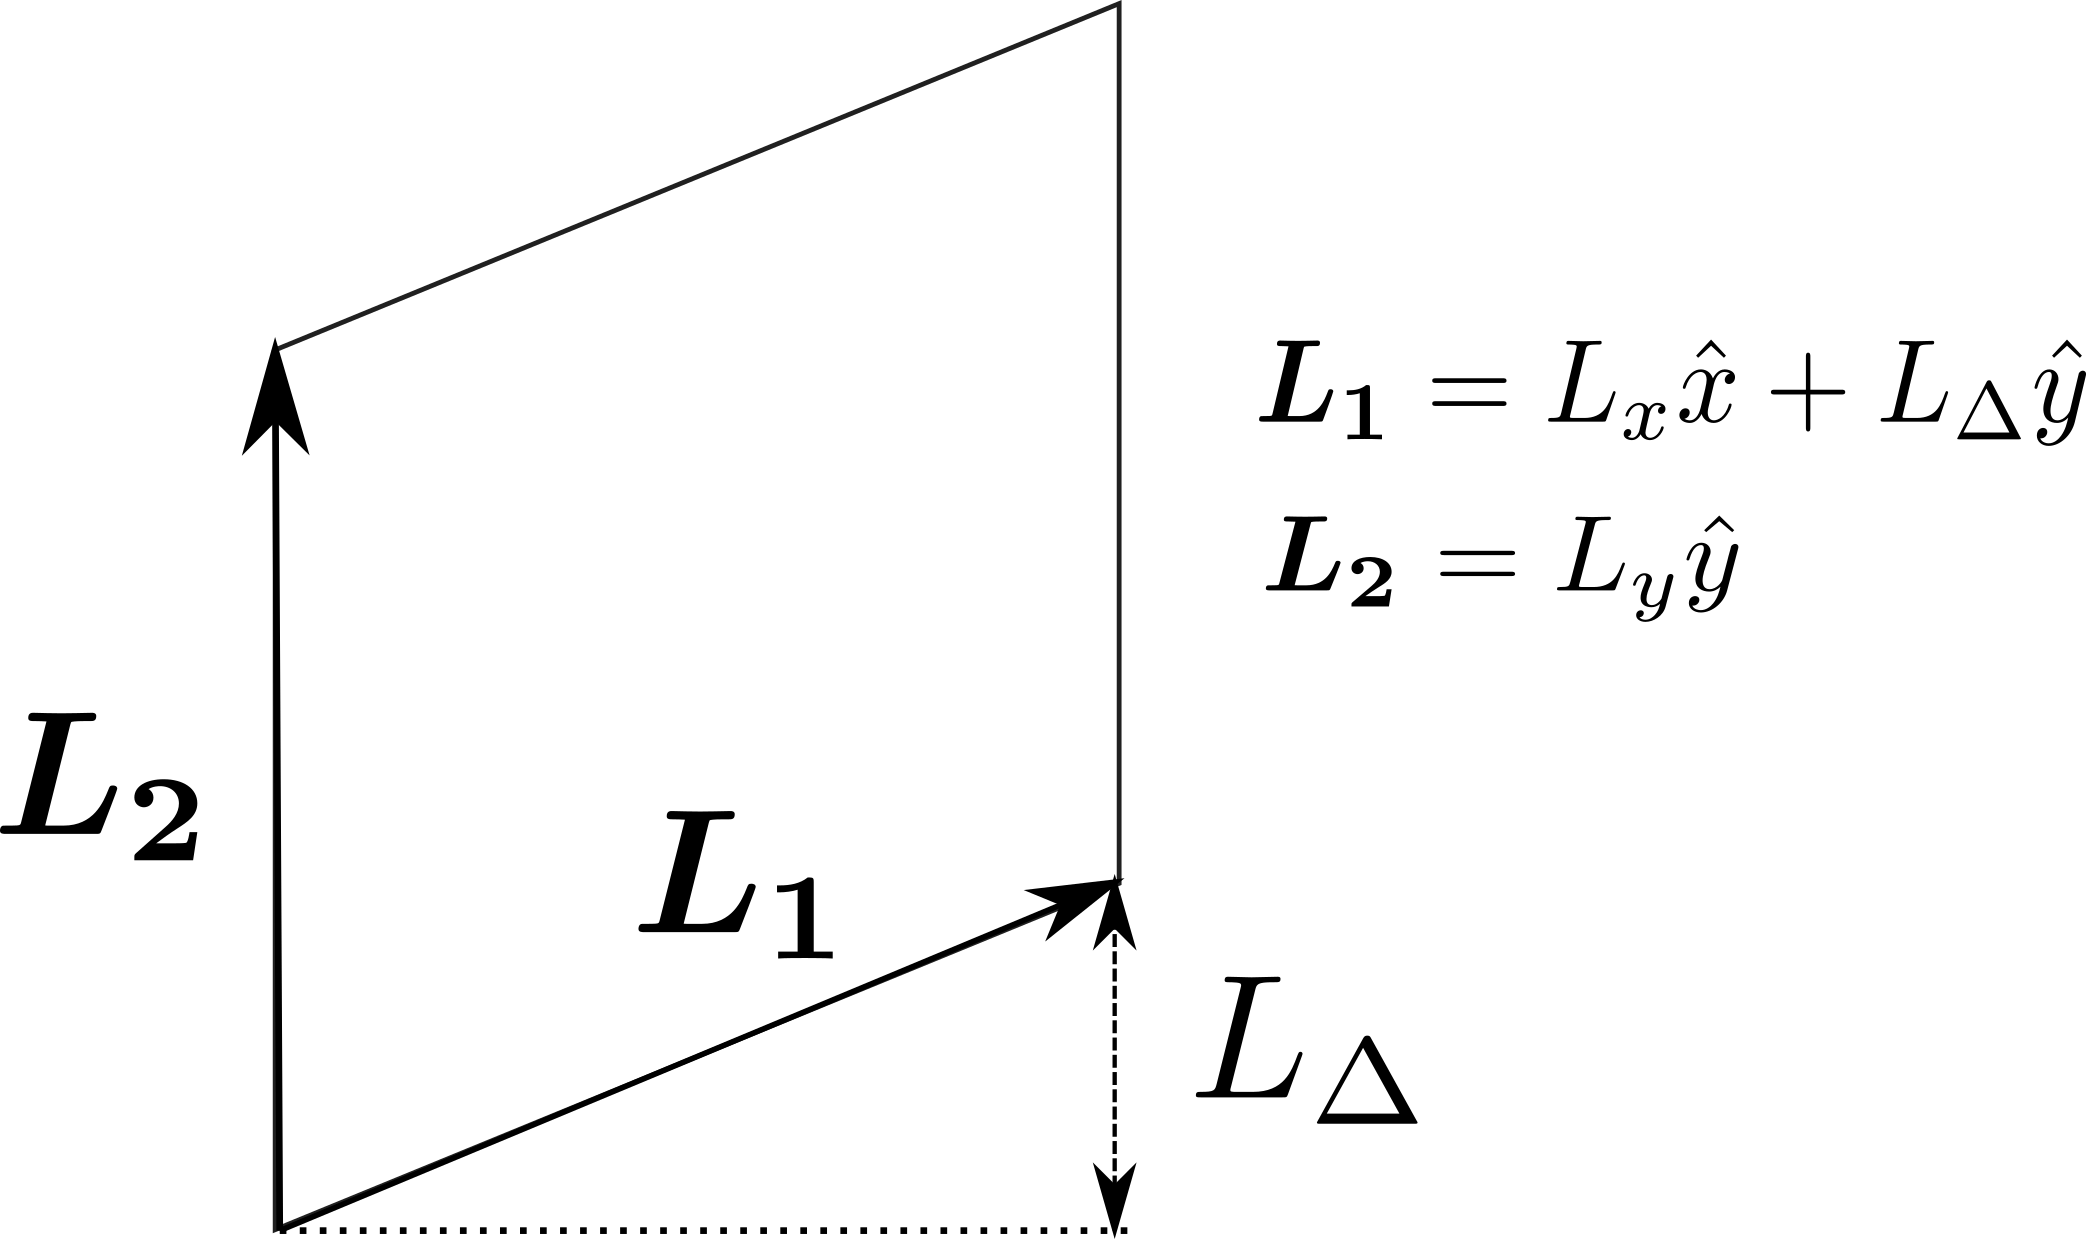
\includegraphics[width=2.5in]{figures/pngs/unit_cell_torus.png}
   			\caption{Unit cell}
    			\label{fig1}
  		\end{figure}

  		Then we demand that the physical observables of the system should not change if any particle(s) is(are) translated 
  		by a vector
  
  		\begin{equation*}
    			\bsym{L_{m,n}} = m\bsym{L_1} + n\bsym{L_2}\quad m,n\in \mathbb{Z}
  		\end{equation*}
  
  			Because such translation brings back the particle in the same position because of imposed pbc. So this 
  			is the first symmetry we have on torus geometry and we will see its implications on a qhe system next.
  	\end{frame}
	
	%===============Intro>MTO====================%

	\begin{frame}[allowframebreaks]{Magnetic Translation Operator}
  		In the absense of magnetic field, the generator of translation is canonical momenta. That is

  		\begin{align}
    			T(\vec{a}) &= \text{exp}\left( \frac{\iota}{\hbar}{\vec{a}\cdot\bsym{P}}\right) \\
    			\implies \quad T(\vec{a})\psi(\vec{x}) &= \psi(\vec{x}+\vec{a}) \non
  		\end{align}
  
  		\framebreak %--------------------------------%
  			  
  		The quantum Hall Hamiltonian looks like 

		\begin{equation}
			H = \sum_{i}\frac{{\bsym{\pi}_{i}}^{2}}{2m}  + \frac{1}{2}\sum_{i,j} V(\vec{r_i}-\vec{r_j})
		\end{equation}
		with $V(\vec{r}_{i,j} + \boldsymbol{L_{m,n}})=V(\vec{r}_{i,j})$ on torus, where $\bsym{\pi}$'s are the 
		physical momenta given as 
		\begin{equation*}
			\bsym{\pi} = \bsym{p} + |e|\bsym{A}(\bsym{r})
		\end{equation*}
		where $\bsym{A}(\bsym{r})$ is the magnetic potential and -ve charge of the electron is accounted for.
	
		\framebreak %--------------------------------%
	
		The interest in translation operator, $T$, is as an accompanying symmetry of $H$ in torus, with a possible 
		reduction of H in smaller sectors corresponding to q-numbers of $T$. But here is a problem : even though, 
		we have canonical momentum commuting with each other
		\begin{equation*}
			[p_x,p_y] = 0
		\end{equation*}
		But physical moments do not commute
		\begin{equation*}
			[\pi_x,\pi_y] \neq 0
		\end{equation*}
		Implying, $[H,\bsym{p}]\neq 0$. Thus translations generated with $\bsym{p}$ or $\bsym{\pi}$ will not 
		commute with $H$.
		
		\framebreak %--------------------------------%
		
		There is a way to remove the non-commuting part from the $\bsym{\pi}$ operators as follows
		
		\begin{align}
			\bsym{K} &= \bsym{\pi} - \frac{\hbar}{l^2}(\hat{z}\times \bsym{r}) \\
			\text{or}\quad \bsym{K} &= \bsym{\pi} - eB(\hat{z}\times \bsym{r}) \non
		\end{align}
		
		such that 
		
		\begin{align*}
			[\bsym{K},\bsym{\pi}]&=0 \\
			\implies\quad [\bsym{K},H]&=0 
		\end{align*}
				
		\framebreak %--------------------------------%
		
		If we make a modified "translation" operator using $\bsym{K}$, as follows
		
		\begin{align}
    			T(\vec{a}) &= \text{exp}\left( \frac{\iota}{\hbar}{\vec{a}\cdot\bsym{K}}\right)
    		\end{align}
		 
		which commutes with $H$, how do we know its action brings the right translation? Else why we are calling 
		it a translation operator at all?
		
		\framebreak %--------------------------------%

		We know
		
		\begin{align}
    			\bsym{K} = \bsym{p} + e\bsym{A}(\bsym{r}) - eB(\hat{z} \times \bsym{r})
    		\end{align}
		
	\end{frame}

	

	\begin{frame}
  		\frametitle{References}
	\end{frame}
\end{document}